%% ============================================================
%%  Memory Controllers for DDR Memories  |  Beamer Presentation
%%  Compile:  pdflatex DDR_MC_Presentation.tex  (run twice)
%% ============================================================
\documentclass[aspectratio=169,10pt]{beamer}

\usetheme{Madrid}
\usecolortheme{default}

%% ── Palette ─────────────────────────────────────────────────
\definecolor{ddrblue}  {RGB}{10,60,100}
\definecolor{ddrteal}  {RGB}{0,130,140}
\definecolor{ddraccent}{RGB}{0,190,180}
\definecolor{ddrgold}  {RGB}{230,170,0}
\definecolor{ddrlight} {RGB}{235,245,250}
\definecolor{ddrred}   {RGB}{180,30,30}
\definecolor{ddrgreen} {RGB}{20,130,80}
\definecolor{ddrgray}  {RGB}{90,100,110}
\definecolor{ddr3col}  {RGB}{26,82,118}
\definecolor{ddr4col}  {RGB}{26,122,74}
\definecolor{ddr5col}  {RGB}{110,43,140}

%% ── Beamer colours ──────────────────────────────────────────
\setbeamercolor{palette primary}  {bg=ddrblue,fg=white}
\setbeamercolor{palette secondary}{bg=ddrteal,fg=white}
\setbeamercolor{palette tertiary} {bg=ddrblue,fg=white}
\setbeamercolor{palette quaternary}{bg=ddrblue,fg=white}
\setbeamercolor{structure}        {fg=ddrblue}
\setbeamercolor{block title}      {bg=ddrblue,fg=white}
\setbeamercolor{block body}       {bg=ddrlight,fg=black}
\setbeamercolor{frametitle}       {bg=ddrblue,fg=white}
\setbeamercolor{title}            {bg=ddrblue,fg=white}

\setbeamerfont{frametitle}{size=\large,series=\bfseries}
\setbeamerfont{title}     {size=\Large,series=\bfseries}

%% ── Packages ────────────────────────────────────────────────
\usepackage{tikz}
\usetikzlibrary{arrows.meta,positioning,shapes.geometric,
                fit,backgrounds,decorations.markings,
                patterns,calc,matrix,chains,decorations.pathreplacing}
\usepackage{pgfplots}
\pgfplotsset{compat=1.18}
\usepackage{booktabs}
\usepackage{colortbl}
\usepackage{xcolor}
\usepackage{amsmath}
\usepackage{siunitx}
\usepackage{microtype}
\usepackage{graphicx}
\usepackage{array}

%% ── TikZ styles ─────────────────────────────────────────────
\tikzset{
  box/.style={rectangle,rounded corners=3pt,draw=#1!70,fill=#1!12,
              text=black,minimum height=7mm,minimum width=22mm,
              font=\footnotesize\bfseries,align=center},
  box/.default=ddrblue,
  arr/.style={-{Stealth[length=5pt]},thick,#1},
  arr/.default=ddrblue,
  phy/.style={rectangle,rounded corners=4pt,draw=ddrteal,
              fill=ddrteal!15,minimum height=8mm,minimum width=24mm,
              font=\footnotesize\bfseries,align=center},
  ddrbox/.style={rectangle,rounded corners=3pt,draw=#1,fill=#1!15,
                 minimum height=7mm,minimum width=20mm,
                 font=\scriptsize\bfseries,align=center},
  imgbox/.style={rectangle,rounded corners=3pt,
                 draw=ddrgray!50,fill=ddrlight,dashed,line width=0.6pt,
                 font=\tiny\itshape,text=ddrgray,align=center,inner sep=4pt},
}

%% ── Image placeholder ───────────────────────────────────────
%% \imgph{width}{height}{filename}  -- shows image if present, box if not
\newcommand{\imgph}[3]{%
  \includegraphics[width=#1,height=#2,keepaspectratio]{#3}%
}

%% ── Header / footer ─────────────────────────────────────────
\setbeamertemplate{navigation symbols}{}
\setbeamertemplate{headline}{%
  \begin{beamercolorbox}[wd=\paperwidth,ht=11ex,dp=1.5ex]{}
    \vspace{3pt}\hfill
    
\includegraphics[height=0.80cm]{images/chips_logo.png}%
    \hspace{0.3cm}
  \end{beamercolorbox}%
}
\setbeamertemplate{footline}{%
  \leavevmode
  \hbox{%
    \begin{beamercolorbox}[wd=\paperwidth,ht=2.25ex,dp=1ex,right]
        {palette tertiary}%
      \usebeamerfont{date in head/foot}%
      \insertframenumber{} / \inserttotalframenumber\hspace{6pt}
    \end{beamercolorbox}}%
  \vskip0pt%
}

\date{}

%% ============================================================
\begin{document}
%% ============================================================

%% ── SLIDE 0 – Title ─────────────────────────────────────────
\begin{frame}[plain]
  \begin{beamercolorbox}[wd=\paperwidth,ht=0.22\paperheight,dp=0pt,
      center,sep=10pt]{frametitle}
    \usebeamerfont{title}\color{white}Memory Controllers for DDR Memories
  \end{beamercolorbox}
  \vspace{20pt}
  \begin{center}
    \begin{tabular}{rl}
      \multicolumn{2}{c}{\textbf{Mentor: Mahesh A}}\\[8pt]
      \textbf{Pranav M}   & \texttt{PES2UG23EC076}\\[6pt]
      \textbf{Lalith}     & \texttt{PES2UG23EC074}\\[6pt]
      \textbf{Harshini S} & \texttt{PES2UG23EC058}\\
    \end{tabular}
  \end{center}
\end{frame}

%% ── SLIDE 1 – Recap ─────────────────────────────────────────
\begin{frame}[fragile]{Recap: Memory Controller for DDR Memories}
\begin{columns}[T]

\begin{column}{0.36\textwidth}
  \vspace{4pt}
  \begin{itemize}\setlength\itemsep{6pt}\small
    \item Acts as a bridge between the SoC and DRAM
    \item Enforces 50+ timing constraints (tWTR, tRC, tFAW\ldots)
    \item Handles row-buffer management and request scheduling
    \item Manages power modes: PASR, TCSR, Deep Power-Down
    \item AXI out-of-order IDs map naturally to DDR bank parallelism
  \end{itemize}
\end{column}

\begin{column}{0.62\textwidth}
  \centering
  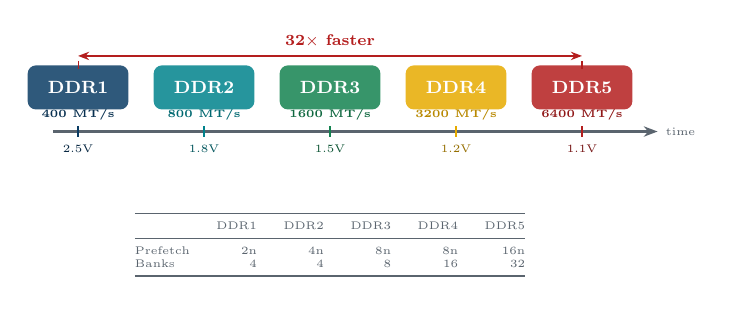
\begin{tikzpicture}[scale=0.80, transform shape]
    \draw[-{Stealth[length=5pt]},thick,ddrgray]
          (-0.4,0)--(9.2,0) node[right,font=\tiny,ddrgray]{time};
    \foreach \gen/\speed/\vdd/\col/\x in {
      DDR1/{400 MT/s}/{2.5V}/ddrblue/0,
      DDR2/{800 MT/s}/{1.8V}/ddrteal/2.0,
      DDR3/{1600 MT/s}/{1.5V}/ddrgreen/4.0,
      DDR4/{3200 MT/s}/{1.2V}/ddrgold/6.0,
      DDR5/{6400 MT/s}/{1.1V}/ddrred/8.0}{
      \node[rectangle,rounded corners=3pt,fill=\col!85,text=white,
            font=\footnotesize\bfseries,minimum width=16mm,minimum height=7mm,
            align=center] at (\x,0.70) {\gen};
      \draw[\col,thick] (\x,0.08)--(\x,-0.08);
      \node[font=\fontsize{5}{6}\selectfont\bfseries,text=\col!80!black]
            at (\x,0.26) {\speed};
      \node[font=\fontsize{5}{6}\selectfont,text=\col!65!black]
            at (\x,-0.28) {\vdd};
    }
    \draw[ddrred,thick,{Stealth[length=4pt]}-{Stealth[length=4pt]}]
      (0,1.20)--node[above,font=\scriptsize\bfseries,ddrred]{32$\times$ faster}
      (8.0,1.20);
    \draw[ddrred,dashed,thin] (0,1.12)--(0,0.98);
    \draw[ddrred,dashed,thin] (8.0,1.12)--(8.0,0.98);
    \node[font=\fontsize{5}{6}\selectfont,align=center,ddrgray]
          at (4.0,-1.8) {%
      \begin{tabular}{@{}lrrrrr@{}}
        \toprule
                 & DDR1 & DDR2 & DDR3 & DDR4 & DDR5\\
        \midrule
        Prefetch & 2n & 4n & 8n & 8n  & 16n\\
        Banks    & 4  & 4  & 8  & 16  & 32 \\
        \bottomrule
      \end{tabular}};
  \end{tikzpicture}
\end{column}
\end{columns}
\end{frame}

%% ── SLIDE 2 – DFI Signal Groups ─────────────────────────────
\begin{frame}[fragile]{DFI Interface: MC \textrightarrow\textleftarrow{} PHY Signal Groups}
\begin{columns}[T]

\begin{column}{0.50\textwidth}
  \centering\vspace{4pt}
  \imgph{0.82\linewidth}{5.2cm}{images/dfi5_2.png}
\end{column}

\begin{column}{0.46\textwidth}
  \vspace{6pt}
  {\small\textbf{\color{ddrblue}Command Interface}}
  \begin{itemize}\setlength\itemsep{1pt}\footnotesize
    \item Address, bank, CS\#, CKE, ODT, RAS\#, CAS\#, WE\#
    \item MC $\to$ PHY; alert feedback PHY $\to$ MC
  \end{itemize}
  \vspace{4pt}
  {\small\textbf{\color{ddrteal}Write Data Interface}}
  \begin{itemize}\setlength\itemsep{1pt}\footnotesize
    \item \texttt{dfi\_wrdata}, \texttt{dfi\_wrdata\_en}, \texttt{dfi\_wrdata\_mask}
    \item CRC and ECC sideband signals
  \end{itemize}
  \vspace{4pt}
  {\small\textbf{\color{ddrgreen}Read Data Interface}}
  \begin{itemize}\setlength\itemsep{1pt}\footnotesize
    \item \texttt{dfi\_rddata\_en} MC $\to$ PHY (look-ahead)
    \item \texttt{dfi\_rddata}, \texttt{dfi\_rddata\_valid} PHY $\to$ MC
  \end{itemize}
  \vspace{4pt}
  {\small\textbf{\color{ddrgold}Update / Status / PHY Managed}}
  \begin{itemize}\setlength\itemsep{1pt}\footnotesize
    \item Handshake: \texttt{ctrlupd}, \texttt{phyupd}, \texttt{phymngd}
    \item Freq ratio, init start/complete, error reporting
  \end{itemize}
\end{column}
\end{columns}
\end{frame}

%% ── SLIDE 3 – Inter-Lane Skew ───────────────────────────────
\begin{frame}[fragile]{Inter-Lane Skew: Off-Die Signal Integrity}
\begin{columns}[T]

\begin{column}{0.38\textwidth}
  \vspace{4pt}
  \begin{itemize}\setlength\itemsep{7pt}\small
    \item DDR transfers data in parallel across multiple DQ byte lanes
    \item Each lane follows a different PCB path, picking up delay $\delta_i$
    \item Skew window: $W_\delta = \max(\delta_i) - \min(\delta_i)$
    \item DDR5 UI $\approx$ 156\,ps; 20\,ps skew eats $>$12\% of it
    \item PHY training (Write Levelling, DQS Gating) corrects $\delta_i$ per lane
  \end{itemize}
\end{column}

\begin{column}{0.58\textwidth}
  \centering\vspace{12pt}
  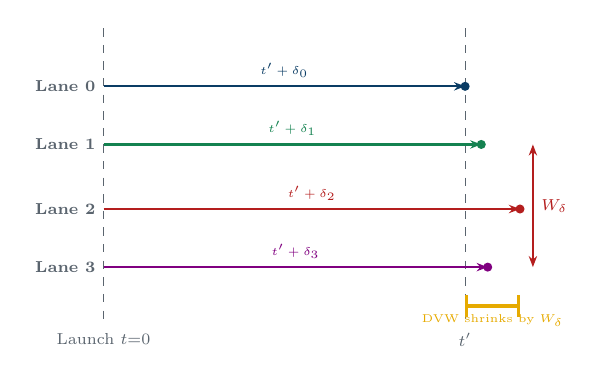
\begin{tikzpicture}[scale=0.82, transform shape]
    \draw[dashed,ddrgray,thin] (0,0.3)--(0,-4.3)
          node[below,font=\scriptsize]{Launch $t{=}0$};
    \draw[dashed,ddrgray,thin] (5.6,0.3)--(5.6,-4.3)
          node[below,font=\scriptsize]{$t'$};
    \foreach \i/\y/\lc/\dx in {
        0/-0.6/ddrblue/0,
        1/-1.5/ddrgreen/0.25,
        2/-2.5/ddrred/0.85,
        3/-3.4/violet/0.35}{
      \node[left,font=\scriptsize\bfseries,ddrgray] at (0,\y) {Lane \i};
      \draw[\lc,thick,-{Stealth[length=4pt]}] (0,\y)
        --node[midway,above,font=\tiny,\lc]{$t'+\delta_\i$}
          (5.6+\dx,\y);
      \fill[\lc] (5.6+\dx,\y) circle (2pt);
    }
    \draw[thick,ddrred,{Stealth[length=4pt]}-{Stealth[length=4pt]}]
          (6.65,-1.5)--node[right,font=\scriptsize,ddrred]{$W_\delta$}
          (6.65,-3.4);
    \draw[ddrgold,very thick,|-|] (5.60,-4.0)--
      node[below,font=\tiny,ddrgold]{DVW shrinks by $W_\delta$}(6.45,-4.0);
  \end{tikzpicture}
\end{column}
\end{columns}
\end{frame}

%% ── SLIDE 4 – Off-Die vs On-Die ─────────────────────────────
\begin{frame}[fragile]{Off-Die vs On-Die Delay}
\begin{columns}[T]

\begin{column}{0.32\textwidth}
  \vspace{2pt}
  {\small\textbf{\color{ddrblue}Off-Die (Picoseconds)}}
  \begin{itemize}\setlength\itemsep{2pt}\small
    \item Signals traverse PCB traces, vias
    \item FR4 velocity $\approx 0.6c$; $\sim$1\,ps per 180\,\si{\micro m}
    \item 30\,mm trace $\approx$ 170\,ps; $W_\delta$ typically 5--50\,ps
  \end{itemize}
  \vspace{5pt}
  {\small\textbf{\color{ddrteal}On-Die (Femto/Attoseconds)}}
  \begin{itemize}\setlength\itemsep{2pt}\small
    \item nm-scale on-chip metal interconnect
    \item 1\,\si{\micro m} wire $\approx$ 3--10\,as propagation
    \item Gate delay (3\,nm): 1--5\,ps; bottleneck is logic depth
  \end{itemize}
  \vspace{5pt}
  {\small\itshape PCB/package is the timing bottleneck, not the silicon.}
\end{column}

\begin{column}{0.64\textwidth}
  \centering\vspace{6pt}
  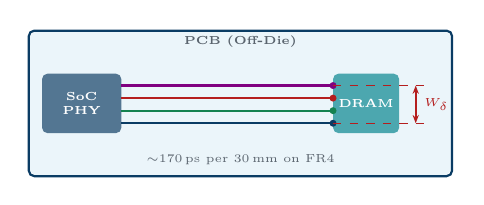
\begin{tikzpicture}[scale=0.84, transform shape]
    \fill[ddrlight,rounded corners=4pt] (0,0) rectangle (6.4,2.2);
    \draw[ddrblue,thick,rounded corners=2pt] (0,0) rectangle (6.4,2.2);
    \node[font=\tiny\bfseries,ddrgray] at (3.2,2.04) {PCB (Off-Die)};
    \fill[ddrblue!70,rounded corners=2pt] (0.2,0.65) rectangle (1.4,1.55);
    \node[white,font=\tiny\bfseries,align=center] at (0.80,1.10) {SoC\\PHY};
    \fill[ddrteal!70,rounded corners=2pt] (4.6,0.65) rectangle (5.6,1.55);
    \node[white,font=\tiny\bfseries] at (5.10,1.10) {DRAM};
    \foreach \y/\col in {0.80/ddrblue,0.99/ddrgreen,1.18/ddrred,1.37/violet}{
      \draw[\col,thick] (1.4,\y)--(4.6,\y);
      \fill[\col] (4.6,\y) circle (1.5pt);
    }
    \draw[{Stealth[length=3pt]}-{Stealth[length=3pt]},ddrred,thick]
         (5.85,0.80)--node[right,font=\tiny,ddrred]{$W_\delta$}(5.85,1.37);
    \draw[ddrred,dashed,thin] (4.6,0.80)--(6.05,0.80);
    \draw[ddrred,dashed,thin] (4.6,1.37)--(6.05,1.37);
    \node[font=\tiny,ddrgray] at (3.2,0.25) {$\sim$170\,ps per 30\,mm on FR4};
  \end{tikzpicture}

  \vspace{8pt}

  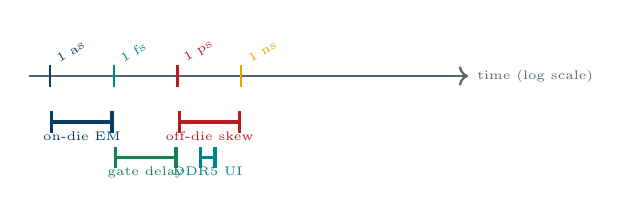
\begin{tikzpicture}[scale=0.90, transform shape]
    \draw[thick,ddrgray,->] (0,0)--(6.2,0)
          node[right,font=\tiny]{time (log scale)};
    \foreach \x/\lab/\col in {
      0.3/{1 as}/ddrblue, 1.2/{1 fs}/ddrteal,
      2.1/{1 ps}/ddrred,  3.0/{1 ns}/ddrgold}{
      \draw[\col,thick] (\x,-0.15)--(\x,0.15);
      \node[\col,font=\tiny,rotate=30,anchor=west] at (\x,0.18) {\lab};
    }
    \draw[ddrblue,very thick,|-|] (0.3,-0.65)
          --node[below,font=\tiny,ddrblue]{on-die EM}(1.2,-0.65);
    \draw[ddrgreen,very thick,|-|] (1.2,-1.15)
          --node[below,font=\tiny,ddrgreen]{gate delay}(2.1,-1.15);
    \draw[ddrred,very thick,|-|] (2.1,-0.65)
          --node[below,font=\tiny,ddrred]{off-die skew}(3.0,-0.65);
    \draw[ddrteal,very thick,|-|] (2.4,-1.15)
          --node[below,font=\tiny,ddrteal]{DDR5 UI}(2.65,-1.15);
  \end{tikzpicture}
\end{column}
\end{columns}
\end{frame}

%% ── SLIDE 5 – Eye Diagram Fundamentals ──────────────────────
\begin{frame}[fragile]{Eye Diagram Fundamentals}
\begin{columns}[T]
\begin{column}{0.48\textwidth}
  \centering\vspace{6pt}
  \imgph{0.75\linewidth}{5.0cm}{images/eye.png}
\end{column}
\begin{column}{0.48\textwidth}
  \vspace{4pt}
  {\small\textbf{\color{ddrblue}Key Regions}}
  \begin{itemize}\setlength\itemsep{4pt}\footnotesize
    \item \textbf{Eye Width:} horizontal opening between transition windows
    \item \textbf{Transition Window:} region where $0{\to}1$ or $1{\to}0$ switching occurs
    \item \textbf{Steady-State Window:} stable HIGH or LOW; sampled here
    \item \textbf{Unit Interval (UI):} one bit period; eye must open within it
  \end{itemize}
  \vspace{6pt}
  {\small\textbf{\color{ddrteal}Why it matters}}
  \begin{itemize}\setlength\itemsep{4pt}\footnotesize
    \item Receiver samples at eye centre for maximum margin
    \item Noise and jitter reduce eye opening
    \item At DDR5-6400: UI $=$ 156\,ps --- any skew directly closes the eye
  \end{itemize}
\end{column}
\end{columns}
\end{frame}

%% ── SLIDE 6 – Trained vs Untrained Eye ──────────────────────
\begin{frame}[fragile]{Eye Diagram: Trained vs Untrained}
\begin{columns}[T]
\begin{column}{0.48\textwidth}
  \centering
  {\small\textbf{\color{ddrred}Untrained Eye}}\\[4pt]
  \imgph{0.55\linewidth}{3.2cm}{images/u_eye.png}\\[4pt]
  \begin{itemize}\setlength\itemsep{3pt}\small
    \item Lane skew $\delta_i$ closes eye horizontally
    \item VREF offset closes eye vertically
    \item ISI and jitter blur transition edges
    \item High BER --- unreliable data capture
  \end{itemize}
\end{column}
\begin{column}{0.48\textwidth}
  \centering
  {\small\textbf{\color{ddrgreen}Trained \& Calibrated Eye}}\\[4pt]
  \imgph{0.55\linewidth}{3.2cm}{images/t_eye.png}\\[4pt]
  \begin{itemize}\setlength\itemsep{3pt}\small
    \item Write Levelling corrects DQS-to-CK skew $\delta_i$
    \item Read centering places sample point at eye centre
    \item ZQ calibration sets correct driver impedance
    \item 2D VREF scan optimises voltage margin $M_V$
  \end{itemize}
\end{column}
\end{columns}
\end{frame}

%% ── SLIDE 7 – Why Picoseconds Matter ────────────────────────
\begin{frame}[fragile]{Why Picoseconds Matter at Modern DDR Speeds}
\begin{columns}[T]

\begin{column}{0.52\textwidth}
  \centering\vspace{4pt}
  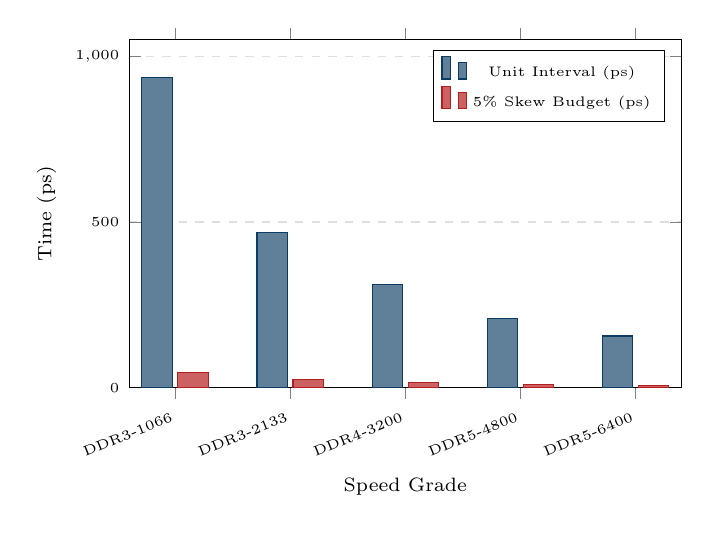
\begin{tikzpicture}
    \begin{axis}[
      ybar, bar width=11pt,
      width=8.6cm, height=6.0cm,
      xlabel={Speed Grade},
      ylabel={Time (ps)},
      xtick={1,2,3,4,5},
      xticklabels={DDR3-1066,DDR3-2133,DDR4-3200,DDR5-4800,DDR5-6400},
      xticklabel style={font=\tiny,rotate=22,anchor=north east},
      yticklabel style={font=\tiny},
      xlabel style={font=\scriptsize},
      ylabel style={font=\scriptsize},
      ymajorgrids=true,
      grid style={dashed,gray!25},
      legend style={font=\tiny,at={(0.97,0.97)},anchor=north east},
      ymin=0, ymax=1050,
    ]
      \addplot[fill=ddrblue!65,draw=ddrblue] coordinates
        {(1,937)(2,469)(3,312)(4,208)(5,156)};
      \addplot[fill=ddrred!70,draw=ddrred] coordinates
        {(1,46.9)(2,23.4)(3,15.6)(4,10.4)(5,7.8)};
      \legend{Unit Interval (ps), 5\% Skew Budget (ps)}
    \end{axis}
  \end{tikzpicture}
\end{column}

\begin{column}{0.44\textwidth}
  \vspace{6pt}
  \centering
  \rowcolors{2}{ddrlight}{white}
  {\footnotesize
  \begin{tabular}{@{}lrr@{}}
    \toprule
    \textbf{Speed} & \textbf{UI} & \textbf{5\% Budget}\\
    \midrule
    DDR3-1066 & 937\,ps & 46.9\,ps\\
    DDR3-2133 & 469\,ps & 23.4\,ps\\
    DDR4-3200 & 312\,ps & 15.6\,ps\\
    DDR5-4800 & 208\,ps & 10.4\,ps\\
    DDR5-6400 & 156\,ps & \textcolor{ddrred}{\textbf{7.8\,ps}}\\
    \bottomrule
  \end{tabular}}

  \vspace{8pt}
  \begin{itemize}\setlength\itemsep{4pt}\small
    \item At DDR5-6400 skew budget is just \textbf{7.8\,ps}
    \item Uncompensated off-die skew can fill this entirely
    \item PHY training trims $\delta_i$ to $\ll$5\,ps per lane
  \end{itemize}
\end{column}
\end{columns}
\end{frame}

%% ── SLIDE 8 – DFI Standard ──────────────────────────────────
\begin{frame}[fragile]{DFI: The Standard MC--PHY Interface}
\begin{columns}[T]

\begin{column}{0.38\textwidth}
  \vspace{4pt}
  \begin{itemize}\setlength\itemsep{7pt}\small
    \item \textbf{DFI} is the industry-standard interface between MC and DDR PHY
    \item Decouples MC from PHY implementation details
    \item Covers command, data, training and power signals
    \item DFI 5.1: PHY-independent boot, expanded freq range, enhanced calibration feedback
  \end{itemize}
\end{column}

\begin{column}{0.58\textwidth}
  \centering\vspace{4pt}
  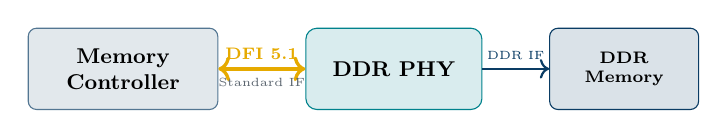
\begin{tikzpicture}[scale=0.86, transform shape]
    \node[box=ddrblue,minimum width=28mm,minimum height=12mm,font=\small\bfseries]
      (mc) at (0,0) {Memory\\Controller};
    \node[phy,minimum width=26mm,minimum height=12mm,font=\small\bfseries]
      (phy) at (4.0,0) {DDR PHY};
    \node[ddrbox=ddrblue,minimum width=22mm,minimum height=12mm]
      (ddr) at (7.4,0) {DDR\\Memory};
    \draw[arr=ddrgold,<->,very thick]
      (mc.east)--node[above,font=\scriptsize\bfseries,ddrgold]{DFI 5.1}
                  node[below,font=\tiny,ddrgray]{Standard IF}(phy.west);
    \draw[arr=ddrblue,->]
      (phy.east)--node[above,font=\tiny]{DDR IF}(ddr.west);
  \end{tikzpicture}

  \vspace{10pt}
  \rowcolors{2}{ddrlight}{white}
  {\scriptsize
  \begin{tabular}{@{}clp{28mm}@{}}
    \toprule
    \textbf{Ver} & \textbf{Key Addition} & \textbf{Support}\\
    \midrule
    1.0 & Initial spec          & DDR, DDR2\\
    2.0 & Training interface    & DDR3, LPDDR2\\
    3.0 & Low-power handshake   & DDR4, LPDDR4\\
    4.0 & DDR4/LPDDR4 paths     & DDR4, LPDDR4\\
    5.0 & PHY-independent boot  & DDR5, LPDDR5\\
    \rowcolor{ddrgold!30}
    \textbf{5.1} & \textbf{Full back-compat} & \textbf{All gens}\\
    \bottomrule
  \end{tabular}}
\end{column}
\end{columns}
\end{frame}

%% ── SLIDE 9 – DFI 5.1 Key Features ─────────────────────────
\begin{frame}[fragile]{DFI 5.1 Key Features}
\begin{columns}[T]

\begin{column}{0.48\textwidth}
  \vspace{4pt}
  {\small\textbf{\color{ddrblue}Three Pillars of DFI 5.1}}
  \begin{enumerate}\setlength\itemsep{7pt}\small
    \item \textbf{PHY-Independent Boot}\\
          MC initialises DRAM without knowing PHY internals
    \item \textbf{Expanded Frequency Range}\\
          Covers low-power LPDDR through DDR5-6400
    \item \textbf{Enhanced PHY$\leftrightarrow$MC Interaction}\\
          Real-time calibration feedback and margining
  \end{enumerate}
\end{column}

\begin{column}{0.48\textwidth}
  \vspace{4pt}
  {\small\textbf{\color{ddrgreen}Backward Compatibility}}
  \begin{itemize}\setlength\itemsep{6pt}\small
    \item Supports DDR through DDR5 and LPDDR through LPDDR5
    \item One DFI 5.1 MC paired with generation-specific PHY covers every standard
  \end{itemize}
  \vspace{8pt}
  {\small\textbf{\color{ddrred}Why it matters for our MC}}
  \begin{itemize}\setlength\itemsep{6pt}\small
    \item Single RTL targets DDR3, DDR4, DDR5 and LPDDR4
    \item Swapping PHY $=$ different memory standard, same controller
  \end{itemize}
\end{column}
\end{columns}
\end{frame}

%% ── SLIDE 10 – JEDEC Comparison Table ───────────────────────
\begin{frame}{DDR3 / DDR4 / DDR5 --- JEDEC Key Specs}
  \vspace{-8pt}
  \centering
  {\scriptsize
  \renewcommand{\arraystretch}{1.15}
  \rowcolors{2}{ddrlight}{white}
  \begin{tabular}{>{\bfseries}p{2.8cm}
                  >{\color{ddr3col}}p{2.9cm}
                  >{\color{ddr4col}}p{2.9cm}
                  >{\color{ddr5col}}p{3.1cm}}
  \rowcolor{ddrblue}
  \textcolor{white}{\textbf{Parameter}} &
  \textcolor{white}{\textbf{DDR3 (JESD79-3F)}} &
  \textcolor{white}{\textbf{DDR4 (JESD79-4C)}} &
  \textcolor{white}{\textbf{DDR5 (JESD79-5B)}} \\
  Data Rate (MT/s)  & 800--2133                  & 1600--3200                & 3200--6400+              \\
  Prefetch / BL     & 8n / BL8 (fixed/fly)       & 8n / BL8 (fixed/fly)      & 16n / BL16 mandatory     \\
  Bank Groups       & None                       & 2 or 4 BGs                & 8 BGs (sub-ch.)          \\
  Channels          & Single                     & Single                    & Sub-channel $\times$2    \\
  IO Voltage        & 1.5\,V / 1.35\,V           & 1.2\,V                    & 1.1\,V                   \\
  On-Die ECC        & Optional                   & Optional                  & Required ($\times$4 org) \\
  Refresh           & tREFI $=7.8\,\mu$s         & tREFI $=7.8\,\mu$s        & Dual-rate / PBR          \\
  Termination       & RTT\_NOM                   & $+$ RTT\_PARK             & $+$ DFITMG               \\
  New timing        & tRCD, tRP, tRAS, tWR, tRFC & $+$ tWTR\_L/S, tRRD\_L/S  & $+$ tRFC1/2/sb, tCS      \\
  \end{tabular}}
\end{frame}

%% ── SLIDE 11 – DDR3 Deep-Dive ───────────────────────────────
\begin{frame}{DDR3 JEDEC Deep-Dive}
  \begin{columns}[T]

    %% LEFT — Timing + MRS
    \begin{column}{0.46\textwidth}
      {\small\textbf{\color{ddr3col}Critical Timing Parameters}}\\[4pt]
      {\footnotesize
      \renewcommand{\arraystretch}{1.2}
      \begin{tabular}{>{\bfseries\color{ddr3col}}l l}
        tRCD & Row open $\to$ column command       \\
        tRP  & Precharge $\to$ next ACT             \\
        tRAS & Min row active time                  \\
        tRC  & tRAS $+$ tRP (full row cycle)        \\
        tWR  & Write $\to$ precharge recovery       \\
        tRFC & Refresh cycle (density-dependent)    \\
        tFAW & 4-bank activation window             \\
        tWTR & Write $\to$ read turnaround          \\
        CL   & CAS latency (cmd $\to$ first data)   \\
      \end{tabular}}

      \vspace{6pt}
      {\small\textbf{\color{ddrteal}Mode Registers (MRS)}}\\[4pt]
      {\footnotesize
      \renewcommand{\arraystretch}{1.2}
      \begin{tabular}{>{\bfseries\color{ddrteal}}l l}
        MR0 & CL, BL, DLL reset, write recovery  \\
        MR1 & Drive strength, RTT\_NOM, AL        \\
        MR2 & CWL, ASR, SRT, RTT\_WR             \\
        MR3 & MPR (multi-purpose register)        \\
      \end{tabular}}
    \end{column}

    %% RIGHT — Init Sequence Flowchart
    \begin{column}{0.50\textwidth}
      {\small\textbf{\color{ddrgold}Initialization Sequence}}\\[4pt]
      \centering
      \begin{tikzpicture}[
        node distance = 0.22cm,
        box/.style = {
          rectangle, rounded corners=3pt,
          draw=ddrblue, fill=ddrlight,
          text width=5.4cm, align=center,
          font=\tiny, inner sep=3pt
        },
        arr/.style = {-Stealth, thick, color=ddrblue}
      ]
        \node[box] (n1) {Stable V\textsubscript{DD} $\ge$ 200\,\textmu s};
        \node[box, below=of n1] (n2) {Assert \texttt{RESET\#} low $\ge$ 200\,\textmu s};
        \node[box, below=of n2] (n3) {De-assert \texttt{RESET\#}; CKE low $\ge$ 500\,\textmu s};
        \node[box, below=of n3] (n4) {Apply stable CK; CKE high after t\textsubscript{XSDLL}};
        \node[box, below=of n4] (n5) {NOP $\ge$ t\textsubscript{XPR} clocks};
        \node[box, below=of n5] (n6) {Load MR2 $\to$ MR3 $\to$ MR1 $\to$ MR0};
        \node[box, below=of n6] (n7) {ZQCL command --- 512 clocks};
        \node[box, below=of n7, fill=ddrgold!20, draw=ddrgold] (n8)
          {\textbf{DRAM ready for normal operation}};
        \foreach \a/\b in {n1/n2, n2/n3, n3/n4, n4/n5, n5/n6, n6/n7, n7/n8}
          \draw[arr] (\a) -- (\b);
      \end{tikzpicture}
    \end{column}

  \end{columns}
\end{frame}

%% ── SLIDE 12 – DDR4 Deep-Dive ───────────────────────────────
\begin{frame}{DDR4 JEDEC Deep-Dive}
  \begin{columns}[T]

    %% LEFT — BG Architecture Diagram
    \begin{column}{0.50\textwidth}
      {\small\textbf{\color{ddr4col}Bank Group Architecture}}\\[4pt]
      \centering
      \scalebox{0.82}{
      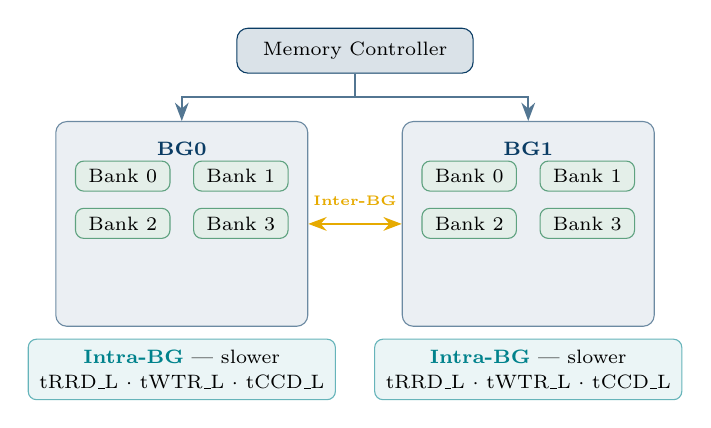
\begin{tikzpicture}[
        every node/.style={font=\scriptsize},
        mc/.style={rectangle, rounded corners=4pt, draw=ddrblue, fill=ddrblue!15,
                   minimum width=3.0cm, align=center, inner sep=5pt},
        bg/.style={rectangle, rounded corners=4pt, draw=ddrblue!60, fill=ddrblue!8,
                   minimum width=3.2cm, minimum height=2.6cm, align=center, inner sep=6pt},
        bank/.style={rectangle, rounded corners=3pt, draw=ddr4col!70, fill=ddr4col!12,
                     minimum width=1.2cm, align=center, inner sep=3pt},
        ann/.style={rectangle, rounded corners=3pt, draw=ddrteal!60, fill=ddrteal!8,
                    minimum width=3.2cm, align=center, inner sep=4pt},
        arr/.style={-Stealth, thick, color=ddrblue!70}
      ]
        % Memory Controller
        \node[mc] (mc) at (0,0) {Memory Controller};

        % BG0 — fixed position left
        \node[bg] (bg0) at (-2.2,-2.2) {};
        \node[font=\scriptsize\bfseries\color{ddrblue}, anchor=north]
          at (bg0.north) [yshift=-4pt] {BG0};
        \node[bank] (b00) at ([xshift=-0.75cm, yshift=-0.7cm] bg0.north) {Bank 0};
        \node[bank] (b01) at ([xshift= 0.75cm, yshift=-0.7cm] bg0.north) {Bank 1};
        \node[bank] (b02) at ([xshift=-0.75cm, yshift=-1.3cm] bg0.north) {Bank 2};
        \node[bank] (b03) at ([xshift= 0.75cm, yshift=-1.3cm] bg0.north) {Bank 3};

        % BG1 — fixed position right
        \node[bg] (bg1) at (2.2,-2.2) {};
        \node[font=\scriptsize\bfseries\color{ddrblue}, anchor=north]
          at (bg1.north) [yshift=-4pt] {BG1};
        \node[bank] (b10) at ([xshift=-0.75cm, yshift=-0.7cm] bg1.north) {Bank 0};
        \node[bank] (b11) at ([xshift= 0.75cm, yshift=-0.7cm] bg1.north) {Bank 1};
        \node[bank] (b12) at ([xshift=-0.75cm, yshift=-1.3cm] bg1.north) {Bank 2};
        \node[bank] (b13) at ([xshift= 0.75cm, yshift=-1.3cm] bg1.north) {Bank 3};

        % MC -> BG arrows
        \draw[arr] (mc.south) -- ++(0,-0.3) -| (bg0.north);
        \draw[arr] (mc.south) -- ++(0,-0.3) -| (bg1.north);

        \draw[{Stealth}-{Stealth}, color=ddrgold, thick]
            (bg0.east) -- (bg1.west);
        \node[font=\tiny\bfseries, color=ddrgold] at (0,-1.9) {Inter-BG};

        % Intra-BG annotations
        \node[ann, anchor=north] at ([yshift=-0.15cm]bg0.south)
          {\textcolor{ddrteal}{\textbf{Intra-BG}} --- slower\\[1pt]
           tRRD\_L $\cdot$ tWTR\_L $\cdot$ tCCD\_L};
        \node[ann, anchor=north] at ([yshift=-0.15cm]bg1.south)
          {\textcolor{ddrteal}{\textbf{Intra-BG}} --- slower\\[1pt]
           tRRD\_L $\cdot$ tWTR\_L $\cdot$ tCCD\_L};

      \end{tikzpicture}}
    \end{column}

    %% RIGHT — PHY Training
    \begin{column}{0.46\textwidth}
      {\small\textbf{\color{ddrgold}PHY Training Procedures}}\\[6pt]
      {\footnotesize
      \begin{enumerate}\setlength\itemsep{5pt}
        \item \textbf{Write Levelling:} DQS launched; DRAM echoes on rising CK; adjusts DQS-to-CK skew per lane
        \item \textbf{Read Gate:} PHY determines preamble window; gates DQS capture
        \item \textbf{Read Centering:} Sweeps DQ VREF; finds eye centre
        \item \textbf{Write Centering:} Tunes PHY DQ delay vs DQS
        \item \textbf{ZQ Cal:} Periodic ZQCS; updates R\textsubscript{ZQ} impedance code
      \end{enumerate}}
    \end{column}

  \end{columns}
\end{frame}

%% ── SLIDE 13 – DDR5 Deep-Dive ───────────────────────────────
\begin{frame}{DDR5 JEDEC Deep-Dive}
  \begin{columns}[T]

    %% LEFT — Sub-channel Architecture Diagram
    \begin{column}{0.50\textwidth}
      {\small\textbf{\color{ddr5col}Sub-Channel Architecture}}\\[6pt]
      \centering
\scalebox{0.80}{
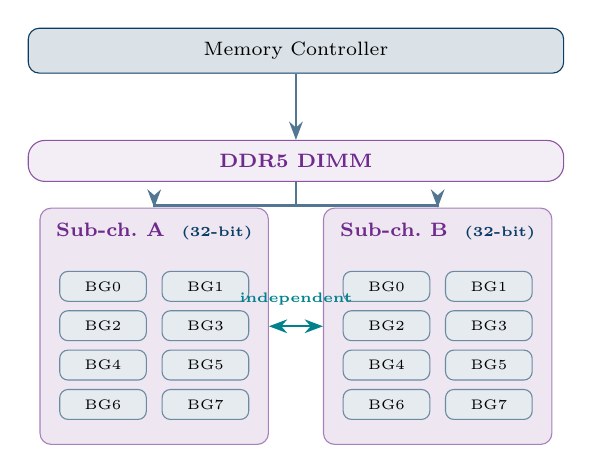
\begin{tikzpicture}[
  every node/.style={font=\scriptsize},
  dimm/.style={rectangle, rounded corners=6pt, draw=ddr5col!80, fill=ddr5col!8,
               minimum width=6.8cm, align=center, inner sep=5pt},
  sch/.style={rectangle, rounded corners=4pt, draw=ddr5col!60, fill=ddr5col!12,
              minimum width=2.9cm, minimum height=3.0cm, align=center, inner sep=5pt},
  bg/.style={rectangle, rounded corners=3pt, draw=ddrblue!60, fill=ddrblue!10,
             minimum width=1.1cm, minimum height=0.38cm, align=center, inner sep=2pt},
  mc/.style={rectangle, rounded corners=4pt, draw=ddrblue, fill=ddrblue!15,
             minimum width=6.8cm, align=center, inner sep=5pt},
  arr/.style={-Stealth, thick, color=ddrblue!70}
]
  \node[mc] (mc) at (0,0) {Memory Controller};
  \node[dimm] (dimm) at (0,-1.4) {\textbf{\color{ddr5col}DDR5 DIMM}};
  \draw[arr] (mc.south) -- (dimm.north);

  \node[sch] (sa) at (-1.8,-3.5) {};
  \node[sch] (sb) at ( 1.8,-3.5) {};

  \draw[arr] (dimm.south) -- ++(0,-0.3) -| (sa.north);
  \draw[arr] (dimm.south) -- ++(0,-0.3) -| (sb.north);

  % Sub-channel labels
  \node[font=\scriptsize\bfseries\color{ddr5col}] at ([yshift=-0.30cm] sa.north)
    {Sub-ch.\ A \ {\color{ddrblue}\tiny(32-bit)}};
  \node[font=\scriptsize\bfseries\color{ddr5col}] at ([yshift=-0.30cm] sb.north)
    {Sub-ch.\ B \ {\color{ddrblue}\tiny(32-bit)}};

  % BG grid SA
  \foreach \row/\dy in {0/-1.0, 1/-1.5, 2/-2.0, 3/-2.5} {
    \node[bg] at ([xshift=-0.65cm, yshift=\dy cm] sa.north) {\tiny BG\the\numexpr\row*2\relax};
    \node[bg] at ([xshift= 0.65cm, yshift=\dy cm] sa.north) {\tiny BG\the\numexpr\row*2+1\relax};
  }

  % BG grid SB
  \foreach \row/\dy in {0/-1.0, 1/-1.5, 2/-2.0, 3/-2.5} {
    \node[bg] at ([xshift=-0.65cm, yshift=\dy cm] sb.north) {\tiny BG\the\numexpr\row*2\relax};
    \node[bg] at ([xshift= 0.65cm, yshift=\dy cm] sb.north) {\tiny BG\the\numexpr\row*2+1\relax};
  }

  % Independent arrow + label
  \node[font=\tiny\bfseries, color=ddrteal] at (0,-3.15) {independent};
  \draw[{Stealth}-{Stealth}, color=ddrteal, thick] (sa.east) -- (sb.west);

\end{tikzpicture}}
    \end{column}

    %% RIGHT — Init & Training
    \begin{column}{0.46\textwidth}
      {\small\textbf{\color{ddrgold}Init \& Training Additions}}\\[6pt]
      {\footnotesize
      \begin{enumerate}\setlength\itemsep{5pt}
        \item \textbf{BCOM training:} Sideband cmd bus trained before main CA bus active
        \item \textbf{PDA mode:} Per-DRAM addressability --- tune MRS per individual device
        \item \textbf{2$\times$ MRS sets:} Extended register space; extra latency $+$ ODT configs
        \item \textbf{RTT\_PARK $+$ DFITMG:} Runtime-switchable ODT via DFI timing params
        \item \textbf{CA parity:} DRAM validates each command frame; error flagged via \texttt{ALERT\_n}
      \end{enumerate}}
    \end{column}

  \end{columns}
\end{frame}
\end{document}
